\documentclass{article}
\usepackage[utf8]{inputenc}
\usepackage[T1]{fontenc}
\usepackage[english]{babel}
\setlength{\parindent}{0pt}
\usepackage{hyperref}
\hypersetup{
    colorlinks=true,
    linkcolor=blue,
    filecolor=magenta,      
    urlcolor=cyan}
\usepackage{graphicx}
\graphicspath{ {./pic/} }
\usepackage{multicol}
\usepackage{lscape}

\usepackage{fourier,amssymb,microtype,amsmath,gensymb}
\newcommand{\R}{\mathbb{R}}
\usepackage{mdframed,caption,xcolor}
\usepackage{tikz,tkz-euclide}

\title{Seminar 5. Production Theory}
\author{Xiaoguang Ling \\  \href{xiaoguang.ling@econ.uio.no}{xiaoguang.ling@econ.uio.no}}
\date{\today}

\begin{document}

\maketitle

%%%%%%%%%%%%%%%%%%%%%%%%%%%%%%%%%%%%%%%%%%%%%%%%%%%%%%%%%%%%%%%%%%%%%%%%%%%%%%%%%%%%%%%%%%%%%%
\begin{landscape}
\section*{Production Duality}


\vspace{3mm}
{\scriptsize
\usetikzlibrary{arrows.meta}
\tikzset{%
  >={Latex[width=1mm,length=1mm]},
  % Specifications for style of nodes:
            base/.style = {rectangle, rounded corners, draw=black,
                           minimum width=2cm, minimum height=1cm,
                           text centered, font=\sffamily},
  Starts/.style = {base, fill=blue!30},
         process/.style = {base, minimum width=2.5cm, fill=orange!15,
                           font=\ttfamily},
}
\begin{tikzpicture}[node distance=2cm,
every node/.style={fill=white, font=\sffamily}, align=center]
\node (start) [Starts] {Profit Maximization: \\ $\max_{(x,y) \ge 0} \ py - wx, s.t. y \le f(x)$};
\node (1) [process, below of=start] {Output Supply Function: \\ $y^* \equiv y(p,w)$ \\ Input Demand Functions: \\ $x^* \equiv x(p,w)$};
\node (2) [process, below of=1] {Profit Function: \\ $\pi (p,w) =  py^* - wx^*$};

\node (3) [process, left of=2,xshift=-1.5cm,yshift=1cm]  {Hotelling's lemma (pp.148): \\ $y(p,w) = \frac{\partial \pi(p,w)}{\partial p}$ \\  \\   $x_i(p,w) = - \frac{\partial \pi(p,w)}{\partial w_i}$};


\draw[->]  (start) -- (1);
\draw[->] (1) -- (2);
\draw[dashed]  (2) --  (3);
\draw[dashed]  (3) --  (1);


{\tiny
\path (start) to  node {Let $y = f(x)$, solution $x^*, y^*$} (1); 
\path (1) to  node {maximized value} (2); 
}
  
%%%%%%%%%%%%%%%%%%%%%%%%%%%%%%%%%%%%%%%%%%%%%%%%%%%%%%%%%%%%%%%%%%%%%%%%%%%%%%%%%%%%%%%%%%%%%%%%%%%%%%%%%%%%%

\node (start2) [Starts, right of = 1, xshift =6cm, yshift=2cm] {Cost Minimization: \\ $\min_{x \in \R^n_+} \ w x, s.t. f(x) \ge y$};
\node (21) [process, below of=start2] {Conditional Input Demand: \\ $x(w,y)$};
\node (22) [process, below of=21] {Cost Function: \\ $c(w,y) = w x(w,y)$};
\node (23) [process, right of=22,xshift=1.5cm,yshift=1cm]  {Shephard's lemma(pp.138): \\ $\frac{\partial c(w^0,y^0)}{\partial w_i} = x_i(w^0,y^0)$};
\node (24) [process, below of=22] {Production Function (pp.144): \\ $f(x) \equiv max\{y \ge 0 | wx \ge c(w,y), \forall w \gg 0 \}$};
\draw[->]  (start2) -- (21);
\draw[->]  (21) -- (22);
\draw[dashed]  (22) --  (23);
\draw[dashed]  (23) --  (21);
\draw[->] (22) --  (24);
{\tiny
\path (start2) to  node {Let $f(x) = y$,solution $x^*$} (21); 
\path (21) to  node {minimized value} (22); 
}
%%%%%%%%%%%%%%%%%%%%%%%%%%%%%%%%%%%%%%%%%%%%%%%%%%%%%%%%%%%%%%%%%%%%%%%%%%%%%%%%%%%%%%%%%%%%%%%%%%%%%%%%%%%%
\node (31) [process, right of=1,xshift=2cm,yshift=0.8cm] {FOC(pp.146): \\ $\frac{\partial f(x^*) / \partial x_i}{\partial f(x^*) / \partial x_j} = \frac{w_i}{w_j}$ \\ Constraint: \\ $f(x) \iff y$};


\draw[<-]  (2) --  (22);
\draw[<->]  (1) --  (21);

\path (22) to  node[above] {$\pi (p,w) = py(p,w) - c(w, y(p,w))$}  (2); 




\end{tikzpicture}
}
\end{landscape}

%%%%%%%%%%%%%%%%%%%%%%%%%%%%%%%%%%%%%%%%%%%%%%%%%%%%%%%%%%%%%%%%%%%%%%%%%%%%%%%%%%%%%%%%%%%%%%

\section{Jehle \& Reny 3.35}

Calculate the \textbf{cost function} and the \textbf{conditional input demands} for the linear production function,
$y = \Sigma^n_{i=1} \alpha_i x_i$.

\begin{mdframed}[backgroundcolor=blue!20,linecolor=white]

\textbf{Production Function}(Jehle \& Reny pp.127)

We use a function $y = f(x)$ to denote $y$ units of a certain commodity is produced using input $x$, where $x \in \R^n_+, y \in \R^1_+$

\vspace{2mm}

\textbf{ASSUMPTION 3.1 Properties of the Production Function} (Jehle \& Reny pp.127)

The production function, $f : \R^n_+ \to \R_+$ , is continuous, strictly increasing, and strictly
quasiconcave on $\R^n_+$, and $f (0) = 0$.

\vspace{2mm}

\textbf{DEFINITION 3.5 The Cost Function} (Jehle \& Reny pp.136)

The cost function, defined for all input prices $w \gg 0$ and all output levels $y \in f(\R^n_+)$ is the
minimum-value function,
$$c(w,y) \equiv \min_{x \in \R^n_+} w \cdot x , \ \ s.t. \ \ f(x) \ge y.$$
The solution $x(w, y)$ is referred to as the firm’s \textbf{conditional input demand}, because it is conditional on the level of output $y$.

\begin{itemize}
\item  \textbf{Conditional input demand} is similar to Hicksian demands for consumers.
\end{itemize}

\end{mdframed}

\vspace{2mm}

\begin{mdframed}[backgroundcolor=blue!20,linecolor=white]

Here the linear production function $y = \Sigma^n_{i=1} \alpha_i x_i$ is very similar to the "\textbf{perfect substitution}" preference in Seminar 4.

\begin{itemize}

\item  The product can be produced by any input $x_i$, the only difference is that for each unit of input, different $x_i$ produces different amount $\alpha_i$ of the output. 

\item  The Marginal Rate of Technical Substitution of input $x_j$ for input $x_i$ is $MRTS_{ij} = \frac{\partial f(x)/ \partial x_i}{\partial f(x)/ \partial x_j} = \frac{\alpha_i}{\alpha_j}$.

\end{itemize}

An example: an apple jam factory has 2 types of input, "single apple ($x_1$)" and "2-apple pack ($x_2$)".

\begin{itemize}
\item With a "single apple", the factory can produce a bottle of apple jam;
\item with a "2-apple pack", 2 bottles.
\item The production function is $y = 1 \cdot x_1 + 2 \cdot x_2$
\end{itemize}

How will the factory choose? Similarly to consumers' preference substitution preference, the factory will spend all money on the "cheapest per unit" input. 

Denote the price for $x_1$ and $x_2$ as $w_1$, $w_2$
\begin{itemize}
\item If $\frac{w_1}{1} = \frac{w_2}{2}$, the factory doesn't care which to use;
\item If $\frac{w_1}{1} < \frac{w_2}{2}$, single apple is cheaper;
\item If $\frac{w_1}{1} > \frac{w_2}{2}$, 2-apple pack is cheaper.
\end{itemize}

\end{mdframed}


Denote the price for input $x_i$  as $w_i$. Define $\omega = min \{\frac{w_1}{\alpha_1}, \frac{w_2}{\alpha_2}, \dots ,\frac{w_n}{\alpha_n}\} $

\vspace{2mm}

If $\omega$ is the price of only one input $x_j$, the firm will only use input $x_j$ to minimize its cost. 

\begin{itemize}
\item Thus $y = \alpha_j x_j$ can minimize the cost, and $x_j = \frac{y}{\alpha_j}$ is the conditional input demands.
\item The cost function $c(w,y) = w_j \frac{y}{\alpha_j} = \omega y$.
\end{itemize}


If $\omega$ is the price of several inputs $x_m, m = 1,2, \dots, M$, the firm can freely combine $x_m$ to minimize its cost, as long as  $\Sigma^M_{m=1} \alpha_m x_m = y$.

\vspace{2mm}

For cost funtion, let's assume $\frac{w_1}{\alpha_1} = \frac{w_2}{\alpha_2}= \dots =\frac{w_M}{\alpha_M} = \omega$, then $\omega$ is the price for $1$ single apple, for example. Again, to produce $y$ bottles of jam, you need the same number of single apples. The cost function is thus $\omega y$

%%%%%%%%%%%%%%%%%%%%%%%%%%%%%%%%%%%%%%%%%%%%%%%%%%%%%%%%%%%%%%%%%%%%%%%%%%%%%%%%%%%%%%%%%%%%%%
\section{Jehle \& Reny 3.46}

\begin{itemize}
\item Verify Theorem 3.7 for the profit function obtained in Example 3.5. 
\item Verify Theorem 3.8 for the associated output supply and input demand functions.
\end{itemize}
%***************************************************
\subsection{Verify Theorem 3.7}

\begin{mdframed}[backgroundcolor=blue!20,linecolor=white]

\textbf{DEFINITION 3.7 The Profit Function} (Jehle \& Reny pp.148)

$$\pi (p,w) \equiv \max_{(x,y) \ge 0} py - wx, \ \ s.t. y \le f(x)$$

\textbf{Note,} $y \le f(x)$ means "you can only decide to produce what's possible to be produced":

\begin{itemize}
\item Assume you want to set an optimal output $y$, forget input $x$ for now;
\item You can "waste", i.e., output $y < f(x)$ is possible. Input is not efficiently used for technology $f(x)$;
\item You can't produce more than what your technology $f(x)$ allows, i.e.  $y \ngtr f(x)$.
\end{itemize}

It's not easy to solve the maximization problem directly because there are 2 variable, $y$ and $x$ (again, $y$ is \textbf{NOT} 
necessarily to be $f(x)$, but it can't exceed $f(x)$).

Since to waste will definitely reduce profit (you have some cost but don't produce anything), you will always avoid wasting by
making fully use of your technology, i.e. $y = f(x)$. Then the profit maximization problem is transformed into:

$$\pi (p,w) = \max_{x \ge 0} p f(x) - wx$$

No constraint anymore! The function has only one variable, input $x$. FOC will solve the problem.


In \textbf{Example 3.5} (Jehle \& Reny pp.151), the CES production function is:

$$y = (x_1^\rho + x_2^\rho)^{\frac{\beta}{\rho}}$$

Where $\beta < 1$ and $0 \ne \rho <1$. To obtain the profit function, we need to solve the maximization problem:


$$\max_{(x,y) \ge 0} py - wx, \ \ s.t. \ \ y \le (x_1^\rho + x_2^\rho)^{\frac{\beta}{\rho}}$$

Again, we don't waste, i.e. $ y = (x_1^\rho + x_2^\rho)^{\frac{\beta}{\rho}}$, the problem above is then:

$$\max_{x \ge 0} p(x_1^\rho + x_2^\rho)^{\frac{\beta}{\rho}} - w_1x_1 - w_2x_2$$

FOC are given in the textbook pp. 151. 

The $y^*$ solved is the \textbf{output supply function}:
\begin{equation}
y^* = (p\beta)^{-\frac{\beta}{\beta - 1}}(w_1^r + w_2^r)^{\frac{\beta}{r(\beta - 1)}}
    \label{eq:E5}   
\end{equation}

(You'll compare the output function with equation \ref{eq:check1} derived from cost minimization.)

The $x^*$ solved is the \textbf{input demand function}:

\begin{equation}
x_i^* = w_i^{\frac{1}{\rho -1}}  (p\beta)^{\frac{-1}{\beta - 1}}(w_1^r + w_2^r)^{\frac{\rho -\beta}{\rho(\beta -1)}}
    \label{eq:E6}   
\end{equation}



The profit function is thus:
\begin{equation}
\pi = py^* - wx^* = p^{-\frac{1}{\beta - 1}} (w_1^r + w_2^r)^{\frac{\beta}{r(\beta - 1)}}\beta^{-\frac{\beta}{\beta - 1}}(1-\beta)
    \label{eq:E7}   
\end{equation}

(You'll compare the profit function with equation \ref{eq:check2} derived from cost minimization.)

\textbf{THEOREM 3.7 Properties of the Profit Function} (Jehle \& Reny pp.148)

If $f$ satisfies Assumption 3.1, then for $p \ge 0$ and $w \ge 0$, the profit function $\pi (p,w)$, where well-defined, is continuous and

\begin{enumerate}

\item Increasing in $p$,
\item Decreasing in $w$,
\item Homogeneous of degree one in $(p,w)$,
\item Convex in $(p,w)$,
\item Differentiable in $(p,w)$.
\item Moreover, under the additional assumption that $f$ is strictly concave \\ (Hotelling's lemma),

$$y(p,w) = \frac{\partial \pi(p,w)}{\partial p},\ and \ \ x_i(p,w) = - \frac{\partial \pi(p,w)}{\partial w_i}. \ \ \ \ i = 1,2, \dots , n.$$
\end{enumerate}
\end{mdframed}

\textbf{1.Increasing in $p$}

For $\pi(p,w) = py^* - wx^* = p^{-\frac{1}{\beta - 1}} (w_1^r + w_2^r)^{\frac{\beta}{r(\beta - 1)}}\beta^{-\frac{\beta}{\beta - 1}}(1-\beta)$,
\begin{align*}
\frac{\partial \pi(p, w)}{\partial p} &= (-\frac{1}{\beta - 1})p^{-\frac{1}{\beta - 1}-1} (w_1^r + w_2^r)^{\frac{\beta}{r(\beta - 1)}}\beta^{-\frac{\beta}{\beta - 1}}(1-\beta) \\
&= p^{\frac{\beta}{1 - \beta}} (w_1^r + w_2^r)^{\frac{\beta}{r(\beta - 1)}}\beta^{-\frac{\beta}{\beta - 1}} \\
&= (p\beta)^{\frac{\beta}{1 - \beta}} (w_1^r + w_2^r)^{\frac{\beta}{r(\beta - 1)}}
\end{align*}

When $0<\beta <1$, $\frac{\partial \pi(p, w)}{\partial p} \ge 0 $

\vspace{3mm}
\textbf{2.Decreasing in $w$}

\begin{align*}
\frac{\partial \pi(p, w)}{\partial w_i} &= 
p^{-\frac{1}{\beta - 1}} [\frac{\beta}{r(\beta - 1)}](w_1^r + w_2^r)^{\frac{\beta}{r(\beta - 1)} -1} r w_i^{r-1}\beta^{-\frac{\beta}{\beta - 1}}(1-\beta) \\
&= p^{-\frac{1}{\beta - 1}} [-\beta](w_1^r + w_2^r)^{\frac{\beta}{r(\beta - 1)} -1} w_i^{r-1}\beta^{-\frac{\beta}{\beta - 1}} \\
&= p^{-\frac{1}{\beta - 1}} [-1](w_1^r + w_2^r)^{\frac{\beta}{\frac{\rho}{\rho -1}(\beta - 1)} -1} w_i^{\frac{\rho}{\rho -1}-1}\beta^{1-\frac{\beta}{\beta - 1}} \\
&= -p^{-\frac{1}{\beta - 1}}(w_1^r + w_2^r)^{\frac{\beta}{\frac{\rho}{\rho -1}(\beta - 1)} -1} w_i^{\frac{1}{\rho -1}}\beta^{-\frac{1}{\beta - 1}} \\
&= -(p\beta)^{-\frac{1}{\beta - 1}}(w_1^r + w_2^r)^{\frac{(\rho -1)\beta}{\rho(\beta - 1)} -1} w_i^{\frac{1}{\rho -1}}\\
&= -(p\beta)^{-\frac{1}{\beta - 1}}(w_1^r + w_2^r)^{\frac{\rho -\beta}{\rho(\beta-1)} }w_i^{\frac{1}{\rho -1}}
\end{align*}

$i = 1,2$.

When $0<\beta <1$, $\frac{\partial \pi(p, w)}{\partial w_i} \le 0 $

\vspace{3mm}
\textbf{3.Homogeneous of degree one in $(p,w)$}

\begin{align*}
\pi(tp,tw) &= (tp)^{-\frac{1}{\beta - 1}} [(tw_1)^r + (tw_2)^r]^{\frac{\beta}{r(\beta - 1)}}\beta^{-\frac{\beta}{\beta - 1}}(1-\beta) \\
&= t^{-\frac{1}{\beta - 1}}p^{-\frac{1}{\beta - 1}} t^{\frac{\beta}{(\beta - 1)}} [(w_1)^r + (w_2)^r]^{\frac{\beta}{r(\beta - 1)}}\beta^{-\frac{\beta}{\beta - 1}}(1-\beta) \\
&= t^{-\frac{1}{\beta - 1} + \frac{\beta}{(\beta - 1)}}p^{-\frac{1}{\beta - 1}} [(w_1)^r + (w_2)^r]^{\frac{\beta}{r(\beta - 1)}}\beta^{-\frac{\beta}{\beta - 1}}(1-\beta) \\
&= tp^{-\frac{1}{\beta - 1}} [(w_1)^r + (w_2)^r]^{\frac{\beta}{r(\beta - 1)}}\beta^{-\frac{\beta}{\beta - 1}}(1-\beta) \\
&= t^1\pi(p,w) 
\end{align*}

\vspace{3mm}
\begin{mdframed}[backgroundcolor=blue!20,linecolor=white]
\textbf{4.Convex in $(p,w)$}
Higher-dimension proof not required in exam

Recall one-dimension condition: 

Convex functions (Jehle \& Reny pp.542):

$f : D \to \R \ $ is a convex function if for all $x^1, x^2 \in D$,

$$f(x^t) \le tf(x^1) + (1 - t)f(x^2), \ \forall t \in [0, 1].$$

Where $x^t \equiv tx^1 + (1-t)x^2, t \in [0,1].$

\vspace{2mm}
{\centering
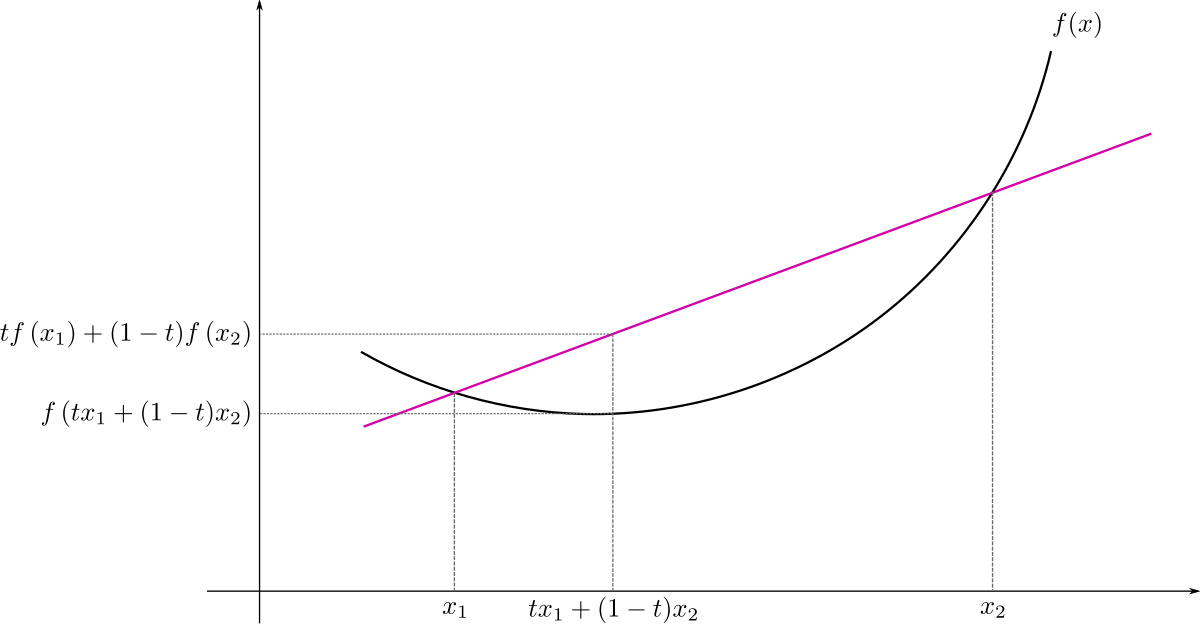
\includegraphics[width=0.8\textwidth]{5.convex}
\captionof{figure}{Convex function}
\label{fig:convex}}
\vspace{2mm}

\textbf{5.Differentiable in $(p,w)$}
Higher-dimension proof not required in exam.

Recall one-dimension condition: derivative exists at $x^0 \Rightarrow$ Differentiable at $x^0$.

\end{mdframed}

\vspace{3mm}
\textbf{6.Hotelling's lemma}

We already calculated the derivatives. Compare them with equation \ref{eq:E5} and \ref{eq:E6}.
%***************************************************
\subsection{Verify Theorem 3.8}

\begin{mdframed}[backgroundcolor=blue!20,linecolor=white]

\textbf{THEOREM 3.8 Properties of Output Supply and Input Demand Functions} (Jehle \& Reny pp.149)

Suppose that $f$ is a strictly concave production function satisfying Assumption 3.1 and that its associated profit function, $\pi(p, y)$, is twice continuously differentiable. Then, for all $p > 0$ and $w \gg 0$ where it is well defined:

\begin{enumerate}

\item Homogeneity of degree zero:
$$y(tp,tw) = y (p,w), \forall t > 0,$$
$$x_i(tp,tw) = x_i(p,w), \forall t > 0 \ and \  i = 1,\dots, n.$$
\item Own-price effects:
$$\frac{\partial y(p,w)}{\partial p} \ge 0,$$
$$\frac{\partial x_i(p,w)}{\partial w_i} \le 0, \ \forall i = 1,\dots, n. $$

\item The substitution matrix is symmetric and positive semidefinite.

\begin{equation}
\left(
    \begin{array}{cccc}
    \frac{\partial y(p,w)}{\partial p} & \frac{\partial y(p,w)}{\partial w_1} & \cdots & \frac{\partial y(p,w)}{\partial w_n} \\
    \frac{\partial x_1(p,w)}{\partial p} & \frac{\partial x_1(p,w)}{\partial w_1} & \cdots & \frac{\partial x_1(p,w)}{\partial w_n} \\
    \vdots    &    \vdots & \ddots &   \vdots \\
    \frac{\partial x_n(p,w)}{\partial p} & \frac{\partial x_n(p,w)}{\partial w_1} & \cdots & \frac{\partial x_n(p,w)}{\partial w_n} \\
    \end{array}
    \right)
\label{eq:subst}   
\end{equation}
\end{enumerate}
\end{mdframed}


Copy from Equation \ref{eq:E5}  and Equation \ref{eq:E6},

\textbf{Output supply function}:
$$
y(p,w) = (p\beta)^{-\frac{\beta}{\beta - 1}}(w_1^r + w_2^r)^{\frac{\beta}{r(\beta - 1)}}
$$

\textbf{Input demand function}:
$$
x_i(p,w) = w_i^{\frac{1}{\rho -1}}  (p\beta)^{\frac{-1}{\beta - 1}}(w_1^r + w_2^r)^{\frac{\rho -\beta}{\rho(\beta -1)}}
$$

\vspace{3mm}
\textbf{1.Homogeneity of degree zero}

\begin{align*}
y(tp,tw) &= (tp\beta)^{-\frac{\beta}{\beta - 1}}[(tw_1)^r + (tw_2)^r]^{\frac{\beta}{r(\beta - 1)}} \\
 &= t^{-\frac{\beta}{\beta - 1}}(p\beta)^{-\frac{\beta}{\beta - 1}} t^{\frac{\beta}{(\beta - 1)}} (w_1^r + w_2^r)^{\frac{\beta}{r(\beta - 1)}} \\
 &=t^0(p\beta)^{-\frac{\beta}{\beta - 1}}(w_1^r + w_2^r)^{\frac{\beta}{r(\beta - 1)}} \\
  &=t^0 y(p,w) 
\end{align*}

\begin{align*}
x_i(tp,tw) &= (tw_i)^{\frac{1}{\rho -1}}  (tp\beta)^{\frac{-1}{\beta - 1}}[(tw_1)^r + (tw_2)^r]^{\frac{\rho -\beta}{\rho(\beta -1)}} \\
&= t^{\frac{1}{\rho -1}} w_i^{\frac{1}{\rho -1}} t^{\frac{-1}{\beta -1}} (p\beta)^{\frac{-1}{\beta - 1}} t^{r\frac{\rho -\beta}{\rho(\beta -1)}} (w_1^r + w_2^r)^{\frac{\rho -\beta}{\rho(\beta -1)}} \\
 &=t^{\frac{1}{\rho -1} + \frac{-1}{\beta -1} + \frac{\rho}{\rho - 1}\frac{\rho -\beta}{\rho(\beta -1)}} w_i^{\frac{1}{\rho -1}}  (p\beta)^{\frac{-1}{\beta - 1}}(w_1^r + w_2^r)^{\frac{\rho -\beta}{\rho(\beta -1)}} \\
  &=t^0 x_i(p,w)
\end{align*}

$i = 1,2$.


\vspace{3mm}
\textbf{2.Own-price effects}

$$\frac{\partial y(p,w)}{\partial p} =(-\frac{\beta}{\beta - 1})p^{-\frac{\beta}{\beta - 1} - 1} (\beta)^{-\frac{\beta}{\beta - 1}}(w_1^r + w_2^r)^{\frac{\beta}{r(\beta - 1)}}$$

When $\beta \in (0,1), \frac{\partial y(p,w)}{\partial p} \ge 0$.


$$\frac{\partial x_i(p,w)}{\partial w_i} =
$$





\vspace{3mm}
\textbf{3.Substitution matrix}



%%%%%%%%%%%%%%%%%%%%%%%%%%%%%%%%%%%%%%%%%%%%%%%%%%%%%%%%%%%%%%%%%%%%%%%%%%%%%%%%%%%%%%%%%%%%%%
\section{Jehle \& Reny 3.49}

\begin{enumerate}
\item Derive the \textbf{cost function} for the production function in Example 3.5 . 

\item Solve $\max_y py - c(w, y)$ 

\item Compare its solution, $y(p,w)$, to the solution in (E.5). Check that $\pi (p,w) = py(p,w) - c(w, y(p,w))$. 

\item Supposing that $\beta > 1$, confirm our conclusion that profits are minimised when the
first-order conditions are satisfied by showing that marginal cost is decreasing at the solution. 

\item Sketch your results.

\end{enumerate}

%***************************************************
\subsection{Cost function}

\begin{mdframed}[backgroundcolor=blue!20,linecolor=white]
CES  production function in Example 3.5 : $y = (x_1^\rho + x_2^\rho)^{\frac{\beta}{\rho}}$, $\beta < 1$ and $0 \ne \rho <1$

Cost function: $c(w,y) \equiv \min_{x \in \R^n_+} w \cdot x , \ \ s.t. \ \ f(x) \ge y.$
\end{mdframed}


$$c(w,y) = \min_{x \in \R^n_+} w_1x_1 + w_2x_2 , \ \ s.t. \ \ (x_1^\rho + x_2^\rho)^{\frac{\beta}{\rho}} \ge y$$

No corner solution.

\begin{itemize}
\item Obviously $x_1,x_2$ can't both be $0$ to produce $y>0$.
\item $\frac{\partial f(x)}{\partial x_i} = \beta (x_1^\rho + x_2^\rho)^{(\frac{\beta}{\rho}) - 1}x_i^{\rho - 1}$. If $\rho \in (0,1),\beta > 0$, $\lim_{x_i \to 0}\frac{\partial f(x)}{\partial x_i} = +\infty$. 
\begin{itemize}
\item If $\rho \in (0,1),\beta < 0$, the production function doesn't make sense since $\lim_{x \to (0,0)} f(x) = + \infty$
\item  If  $\rho < 0$, the production function is not defined at $x_i = 0$
\end{itemize}

\item $f(x) = y$ is binding: $f(x)$ is increasing in $x$, to reduce cost, we shouldn't produce more than required ($y$).
\end{itemize}

$$L =  w_1x_1 + w_2x_2 + \lambda [y -  (x_1^\rho + x_2^\rho)^{\frac{\beta}{\rho}}] $$ 

FOC:

\begin{equation}
    \begin{cases}
\frac{\partial L}{\partial x_1} =w_1 - \lambda \beta (x_1^\rho + x_2^\rho)^{(\frac{\beta}{\rho}) - 1}x_1^{\rho - 1}= 0 \\
\frac{\partial L}{\partial x_2} =w_2 - \lambda \beta (x_1^\rho + x_2^\rho)^{(\frac{\beta}{\rho}) - 1}x_2^{\rho - 1} = 0 \\
y -  (x_1^\rho + x_2^\rho)^{\frac{\beta}{\rho}} = 0
    \end{cases}
    \nonumber
\end{equation}

Simplify:

\begin{equation}
    \begin{cases}
 w_1 = \lambda \beta (x_1^\rho + x_2^\rho)^{(\frac{\beta}{\rho}) - 1}x_1^{\rho - 1} \\
 w_2 =\lambda \beta (x_1^\rho + x_2^\rho)^{(\frac{\beta}{\rho}) - 1}x_2^{\rho - 1} \\
(x_1^\rho + x_2^\rho)^{\frac{\beta}{\rho}} = y
    \end{cases}
    \label{eq:3_49_foc}   
\end{equation}

Taking the ratio between the first two gives:

$$\frac{w_1}{w_2}= (\frac{x_1}{x_2})^{\rho - 1} \Rightarrow x_1 = (\frac{w_1}{w_2})^{\frac{1}{\rho - 1}} x_2$$

Substituting in the third gives:

\begin{align*}
\{[(\frac{w_1}{w_2})^{\frac{1}{\rho - 1}} x_2]^\rho + x_2^\rho\}^{\frac{\beta}{\rho}} &=y \\
[(\frac{w_1}{w_2})^{\frac{\rho}{\rho - 1}} x_2^\rho + x_2^\rho]^{\frac{\beta}{\rho}} &=y \\
[(\frac{w_1}{w_2})^{\frac{\rho}{\rho - 1}} + 1]^{\frac{\beta}{\rho}} x_2^\beta &=y \\
x_2 &= (\frac{y}{[(\frac{w_1}{w_2})^{\frac{\rho}{\rho - 1}} + 1]^{\frac{\beta}{\rho}} })^{\frac{1}{\beta}} \\
 &= y^{\frac{1}{\beta}} [\frac{1}{(\frac{w_1}{w_2})^{\frac{\rho}{\rho - 1}} + 1}]^{\frac{1}{\rho}} \\
&= y^{\frac{1}{\beta}} [\frac{1}{(\frac{w_1}{w_2})^{\frac{\rho}{\rho - 1}} + 1}]^{\frac{1}{\rho}} \\
&= y^{\frac{1}{\beta}} (\frac{w_2^{\frac{\rho}{\rho - 1}}}{w_1^{\frac{\rho}{\rho - 1}} + w_2^{\frac{\rho}{\rho - 1}}})^{\frac{1}{\rho}} \\
\Rightarrow x_1 &= (\frac{w_1}{w_2})^{\frac{1}{\rho - 1}} x_2  \\
&= y^{\frac{1}{\beta}} (\frac{w_1^{\frac{\rho}{\rho - 1}}   }{w_2^{\frac{\rho}{\rho - 1}}   } \frac{w_2^{\frac{\rho}{\rho - 1}}}{w_1^{\frac{\rho}{\rho - 1}} + w_2^{\frac{\rho}{\rho - 1}}})^{\frac{1}{\rho}}  \\
&=y^{\frac{1}{\beta}} (\frac{w_1^{\frac{\rho}{\rho - 1}}}{w_1^{\frac{\rho}{\rho - 1}} + w_2^{\frac{\rho}{\rho - 1}}})^{\frac{1}{\rho}} 
\end{align*}

Cost function: 
\begin{align*}
c(w,y) = w_1x_1 + w_2x_2 &= w_1y^{\frac{1}{\beta}} (\frac{w_1^{\frac{\rho}{\rho - 1}}}{w_1^{\frac{\rho}{\rho - 1}} + w_2^{\frac{\rho}{\rho - 1}}})^{\frac{1}{\rho}}  +w_2 y^{\frac{1}{\beta}} (\frac{w_2^{\frac{\rho}{\rho - 1}}}{w_1^{\frac{\rho}{\rho - 1}} + w_2^{\frac{\rho}{\rho - 1}}})^{\frac{1}{\rho}} \\
&= w_1y^{\frac{1}{\beta}} \frac{w_1^{\frac{1}{\rho - 1}}}{(w_1^{\frac{\rho}{\rho - 1}} + w_2^{\frac{\rho}{\rho - 1}})^{\frac{1}{\rho}}}  +w_2 y^{\frac{1}{\beta}} \frac{w_2^{\frac{1}{\rho - 1}}}{(w_1^{\frac{\rho}{\rho - 1}} + w_2^{\frac{\rho}{\rho - 1}})^{\frac{1}{\rho}}} \\
&=y^{\frac{1}{\beta}} [\frac{w_1^{(\frac{1}{\rho - 1}+1)}}{(w_1^{\frac{\rho}{\rho - 1}} + w_2^{\frac{\rho}{\rho - 1}})^{\frac{1}{\rho}}} + \frac{w_2^{(\frac{1}{\rho - 1}+1)}}{(w_1^{\frac{\rho}{\rho - 1}} + w_2^{\frac{\rho}{\rho - 1}})^{\frac{1}{\rho}}}] \\
&=y^{\frac{1}{\beta}}\frac{w_1^r+w_1^r}{(w_1^r + w_2^r)^{\frac{1}{\rho}}} \\
&=y^{\frac{1}{\beta}}{(w_1^r + w_2^r)^{1 - \frac{1}{\rho}}} \\
&=y^{\frac{1}{\beta}}{(w_1^r + w_2^r)^{\frac{1}{r}}} \\
\end{align*}

Where $r = \frac{\rho}{\rho -1}$

%***************************************************
\subsection{Solve $\max_y py - c(w, y)$ }

$$py - c(w, y) = py - y^{\frac{1}{\beta}}{(w_1^r + w_2^r)^{\frac{1}{r}}} $$

FOC:

$$\frac{d(py - y^{\frac{1}{\beta}}{(w_1^r + w_2^r)^{\frac{1}{r}}})}{dy}= p - \frac{1}{\beta}y^{\frac{1}{\beta} - 1} (w_1^r + w_2^r)^{\frac{1}{r}} = 0$$

\begin{equation}
\therefore y^{\frac{1- \beta}{\beta}} = p \beta (w_1^r + w_2^r)^{-\frac{1}{r}}  \Rightarrow y =  (p \beta)^{\frac{\beta}{1- \beta}} (w_1^r + w_2^r)^{^{\frac{\beta}{r(\beta - 1)}}}
    \label{eq:check1}   
\end{equation}

%***************************************************
\subsection{Check $\pi (p,w) = py(p,w) - c(w, y(p,w))$}

\textbf{1.output function}

Compare the output function \ref{eq:check1} with \ref{eq:E5}, the results are the same.

\textbf{1.Profit function}

\begin{align}
\begin{split}
py(p,w) - c(w, y(p,w)) &= p[(p \beta)^{\frac{\beta}{1- \beta}} (w_1^r + w_2^r)^{^{\frac{\beta}{r(\beta - 1)}}}] \\ 
&\ \ \ \ \ \ \ \ - [(p \beta)^{\frac{\beta}{1- \beta}} (w_1^r + w_2^r)^{^{\frac{\beta}{r(\beta - 1)}}}]^{\frac{1}{\beta}}{(w_1^r + w_2^r)^{\frac{1}{r}}} \\
&= p^{\frac{1}{1- \beta}} \beta^{\frac{\beta}{1- \beta}}(w_1^r + w_2^r)^{^{\frac{\beta}{r(\beta - 1)}}} \\ 
&\ \ \ \ \ \ \ \ - (p\beta)^{\frac{1}{1- \beta}} (w_1^r + w_2^r)^{\frac{1}{r(\beta - 1)}}(w_1^r + w_2^r)^{\frac{1}{r}} \\
&= p^{\frac{1}{1- \beta}} \beta^{\frac{\beta}{1- \beta}}(w_1^r + w_2^r)^{^{\frac{\beta}{r(\beta - 1)}}} - (p\beta)^{\frac{1}{1- \beta}} (w_1^r + w_2^r)^{\frac{\beta}{r(\beta - 1)}} \\
&= [p^{\frac{1}{1- \beta}} \beta^{\frac{\beta}{1- \beta}} - (p\beta)^{\frac{1}{1- \beta}}] (w_1^r + w_2^r)^{\frac{\beta}{r(\beta - 1)}} \\
&= [p^{\frac{1}{1- \beta}} \beta^{\frac{\beta}{1- \beta}} - p^{\frac{1}{1- \beta}} \beta^{\frac{1}{1- \beta}}] (w_1^r + w_2^r)^{\frac{\beta}{r(\beta - 1)}} \\
&= [ \beta^{\frac{\beta}{1- \beta}} -\beta^{\frac{1}{1- \beta}}] p^{\frac{1}{1- \beta}}(w_1^r + w_2^r)^{\frac{\beta}{r(\beta - 1)}} \\
&= [ 1 -\beta^1] \beta^{\frac{\beta}{1- \beta}} p^{\frac{1}{1- \beta}}(w_1^r + w_2^r)^{\frac{\beta}{r(\beta - 1)}} \\
&= p^{\frac{1}{1- \beta}}(w_1^r + w_2^r)^{\frac{\beta}{r(\beta - 1)}} \beta^{\frac{\beta}{1- \beta}}(1 -\beta^1)
\end{split}
\label{eq:check2}   
\end{align}

Compare the result \ref{eq:check2} with the profit function \ref{eq:E7} obtained from profit maximization problem.

\begin{center}
\textbf{Profit maximization $\iff$  Cost minimization}
\end{center}

%***************************************************
\subsection{Marginal Cost and output}

\begin{mdframed}[backgroundcolor=blue!20,linecolor=white]

We already know the cost function given output $y$:
$$c(w,y) = y^{\frac{1}{\beta}}{(w_1^r + w_2^r)^{\frac{1}{r}}} $$

Forget that we already know \textbf{Profit maximization $\iff$  Cost minimization} for now.

To maximize our profit, we want instead the difference between $py$ and $c(w,y)$(the least cost for every given $y$) to be as big as possible,i.e.:
$$\max_{y} py - c(w,y)$$

As a price receiver (competitive firm), how should we change $y$ to achieve this?

FOC:
$$\frac{d(py - c(w,y))}{dy} = p - \frac{dc(w,y)}{dy}=0$$

SOC:

$$\frac{d^2(py - c(w,y))}{dy^2} = - \frac{d^2c(w,y)}{dy^2} \le 0 \Rightarrow \frac{d^2c(w,y)}{dy^2} \ge 0$$

Figure \ref{fig:soc} is a very nice plot showing why FOC is not enough for "maximum poit":

\vspace{2mm}
{\centering
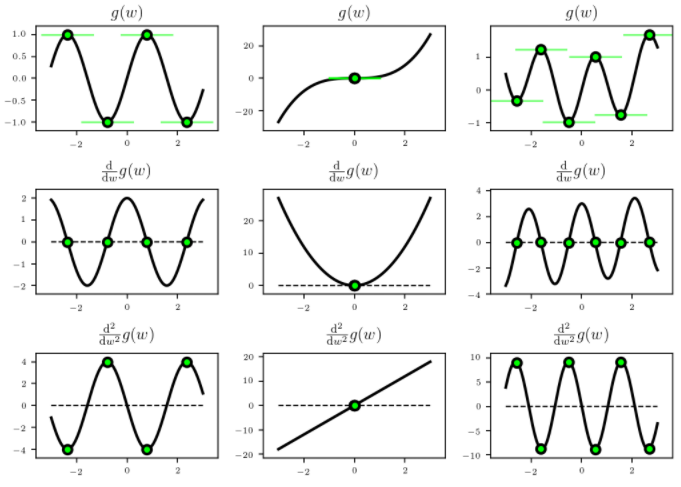
\includegraphics[width=0.8\textwidth]{5.soc}
\captionof{figure}{Second order condition}
\label{fig:soc}}
\vspace{2mm}

(The Figure is from \href{https://kenndanielso.github.io/mlrefined/blog_posts/7_Second_order_methods/7_8_Second_order_condition.html}{Intuiting the condition by example})


We choose the level $y^*$ of output such that 
$$\frac{dc(w,y)}{dy}= p$$
(Marginal cost = price). And,
$\frac{d^2c(w,y)}{dy^2} \ge 0$
(Marginal cost increasing in scale)

\vspace{2mm}
{\centering
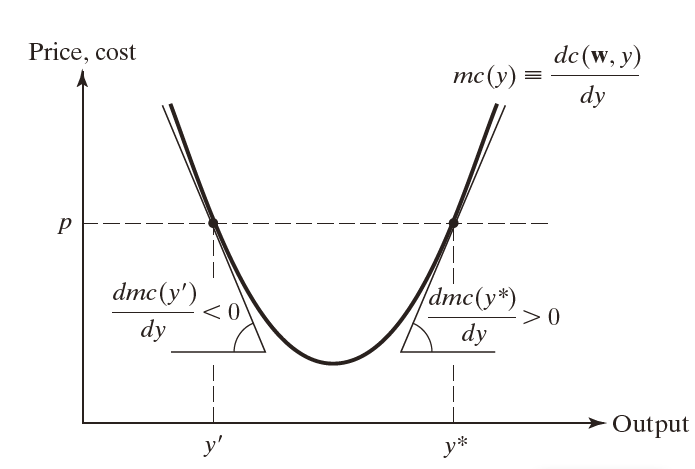
\includegraphics[width=0.8\textwidth]{5.mc}
\captionof{figure}{Marginal cost and price}
\label{fig:mc}}
\vspace{2mm}

\end{mdframed}

Given $c(w,y) = y^{\frac{1}{\beta}}{(w_1^r + w_2^r)^{\frac{1}{r}}} $,

$$MC=\frac{dc(w,y)}{dy}= \frac{1}{\beta}  y^{\frac{1}{\beta} - 1}{(w_1^r + w_2^r)^{\frac{1}{r}}}$$

$$\frac{d MC}{dy} = \frac{1}{\beta}(\frac{1}{\beta} - 1)  y^{\frac{1}{\beta} - 2}{(w_1^r + w_2^r)^{\frac{1}{r}}}$$


If $\beta >1$, $\frac{d MC}{dy} < 0$. The solution is therefore minimized profit, instead of maximized profit.

\begin{mdframed}[backgroundcolor=blue!20,linecolor=white]
Intuitively, $MC=\frac{1}{\beta}  y^{\frac{1}{\beta} - 1}{(w_1^r + w_2^r)^{\frac{1}{r}}}$ is decreasing in $y$ when $\beta > 1$, the more you produce, the less cost you need to pay for 1 more unit output. You will therefore continue to produce $+\infty$.
\end{mdframed}

%***************************************************
\subsection{Sketch}

\begin{center}
\begin{tikzpicture}[scale=1]
\draw[thick,<->] (0,7) node[left]{$\$$}--(0,0)--(10,0) node[right]{$y$};
\node [below left] at (0,0) {$0$};
\draw(1,6) ..controls (2,5) and (5,3).. (9,3) node[right]{$MC$};
\draw [blue] (0,4)--(10,4) ;
\draw (4.16,0)--(4.16,4) ;
\node[left,blue] at (0,4) {$p$} ;
\node[below] at (4.16,0) {$y^*$} ;

\end{tikzpicture}
\captionof{figure}{Decreasing MC and p}
\label{fig:mc}
\end{center}
\vspace{2mm}

If you stop at $y^*$, you lose the most!

\end{document}
